\documentclass[12pt]{article}
\usepackage{amsmath}
\usepackage{amssymb}
\usepackage{listings}             % Include the listings-package
\usepackage{graphicx}
\usepackage{setspace}
\usepackage{float}
\restylefloat{table}
\onehalfspacing

\begin{document}

\title{Catalan Structures and their Bijections}
\author{Stuart Paton}

\maketitle
\thispagestyle{empty}

\pagenumbering{arabic}

\begin{Abstract}
There are more that 100 combinatorial structures whose cardinalities are given by the so called Catalan numbers. The examples used are permutations of $\mathfrak{S}_3$, Dyck Paths, Young Tableaux and triangulations of an $n+2$-gon.\\
On the surface, these structures are very different, but being equinumerous there must be one-to-one correspondences that allows us 
to translate between them. In this project we study commonalities shared by Catalan structures by programming one-to-one 
correspondences. We do this in a systematic way by recursively decomposing the structures. The actual one-to-one correspondences are 
then automatically derived, given the decompositions. Finally we visualise each structure in our application which converts between each Catalan structure.\\ 
From this point we then analyse the bijections from a base set of combinatorial statistics and report our findings from the evaluation of statistics. 
\end{Abstract}
\clearpage

%%%%%%%%%%%%%%%%%%%%%%%%%%%%%%%%%%%%%%%%%%%%%%%%%%%%%%%%%%%%%%%%%%%%%%%%%%%%%%%%%%%
%	Acknowledgements
%%%%%%%%%%%%%%%%%%%%%%%%%%%%%%%%%%%%%%%%%%%%%%%%%%%%%%%%%%%%%%%%%%%%%%%%%%%%%%%%%%%
\par
{\\ \centering{\bf{Acknowledgements} \\}}
I would like to thank my project supervisor Dr Anders Claesson for all the help and support he gave me throughout this project. I would also like to thank Dr Sergey Kitaev for the constructive feedback given at the poster presentation.
\clearpage

\tableofcontents
\newpage


%%%%%%%%%%%%%%%%%%%%%%%%%%%%%%%%%%%%%%%%%%%%%%%%%%%%%%%%%%%%%%%%%%%%%%%%%%%%%%%%%%%
%	Introduction
%%%%%%%%%%%%%%%%%%%%%%%%%%%%%%%%%%%%%%%%%%%%%%%%%%%%%%%%%%%%%%%%%%%%%%%%%%%%%%%%%%%
\section{Introduction}
Catalan structures are combinatorial structures which satisfy the recurrence relation of the $nth$ Catalan number, $c_n$;
\begin{equation}
c_{n} = c_{0}c_{n-1} + c_{1}c_{n-2} + ... + c_{n-1}c_{0}
\end{equation} 
where $c_0 = 1$ and $c_1 = 1$. For $n \geq 1$ we have $c_n = (^{2n}_{n})/(n+1)$. \cite{McShine_onThe}\\
All Catalan structures are equinumerous in the respect that they all have the same cardinality, and are hence equivalent as they satisfy the recurrence relation above.\\
In this project, I looked at a small amount of Catalan structures and evaluated their generating functions and modelled each structure in Haskell, and allowed the user to convert between them using known bijections. Finally graphics for each structure was modelled allowing the user the capabilities of visualising each structure on screen.

\subsection{Report Structure}
This report will be structured in the following format. Chapter 1 provides a description of the aims and scope of this project and a brief summary for the structure of this report. Chapter 2 will provide a literature review where other work in this field will be surveyed and critically reviewed. The next few chapters will contain details into the design of the project where each combinatorial structure will be discussed and the design of the system will be discussed in detail. Finally the evaluation will be discussed fully within the final two chapters.

%%%%%%%%%%%%%%%%%%%%%%%%%%%%%%%%%%%%%%%%%%%%%%%%%%%%%%%%%%%%%%%%%%%%%%%%%%%%%%%%%%%
%	Related Work
%%%%%%%%%%%%%%%%%%%%%%%%%%%%%%%%%%%%%%%%%%%%%%%%%%%%%%%%%%%%%%%%%%%%%%%%%%%%%%%%%%%
\section{Survey of Related Work}
In this chapter a survey of related work will be carried out in the field of enumerative combinatorics surrounding Catalan structures. Many academic papers and books were used to develop a sound understanding of the field and enable the project to be carried out. In the chapter named Combinatorial Structures, there is a discussion on each Catalan structure used.\\

\subsection{Summary of "On the Mixing Time of the Triangulation and Other Catalan Structures}
The first paper that will be discussed is "On the Mixing Time of the Triangulation Walk and other Catalan Structures" by Lisa McShine and Prasad Tetali.\cite{McShine_onThe} This is the key paper that was used to develop an insight to what a Catalan structure is, and some structures which are used throughout this project. The paper describes the amount of steps necessary to generate a triangulation of a convex $n$-gon uniformly at random.\\
In section 2 of this paper, Catalan structures were introduced to the reader as a recurrence relation which the $nth$ Catalan number, $c_n$ satisfies. The problems of triangulations of an $n+2$-gon, and Dyck paths are also introduced to the reader by simply stating the problem. A triangulation of an $n+2$-gon is a dissection of a convex polygon with $n+2$ diagonals using non-intersecting diagonals of the same polygon. In the paper a Dyck path is introduced as a lattice path with steps of $(1,1)$ and $(1,-1)$ which never fall below the $x-$axis. 

%%%%%%%%%%%%%%%%%%%%%%%%%%%%%%%%%%%%%%%%%%%%%%%%%%%%%%%%%%%%%%%%%%%%%%%%%%%%%%%%%%%
%	Combinatorial Structures
%%%%%%%%%%%%%%%%%%%%%%%%%%%%%%%%%%%%%%%%%%%%%%%%%%%%%%%%%%%%%%%%%%%%%%%%%%%%%%%%%%%
\section{Combinatorial Structures}
In this chapter we will be analysing each structure which is being analysed and evaluated within this report.

%%%%%%%%%%%%%%%%%%%%%%%%%%%%%%%%%%%%%%%%%%%%%%%%%%%%%%%%%%%%%%%%%%%%%%%%%%%%%%%%%%%
%	Combinatorial Structures - Dyck Paths
%%%%%%%%%%%%%%%%%%%%%%%%%%%%%%%%%%%%%%%%%%%%%%%%%%%%%%%%%%%%%%%%%%%%%%%%%%%%%%%%%%%
\subsection{Dyck Paths}
A Dyck path of length $2n$ is a lattice path from $(0,0)$ to $(2n, 0)$ with steps:\\
\begin{equation}
\begin{split}
u = (1,1)\\
d = (1, -1)\\
\end{split}
\end{equation}
that never go below the $x$-axis.\\
\\
We can see that if $D$ denotes the set of all Dyck paths then one has the following relation for $D$:\\
\begin{equation}
\begin{split}
$D = 1 + udD + uDdD$
\end{split}
\end{equation}
but since the first path does not have to have its first pattern as $ud$
%singleTree.jpeg\\
%\begin{figure}[h!]
%  \centering
%    \includegraphics[width=0.5\textwidth]{singleTree}
%\end{figure}
then we can generalise to\\
\begin{equation}
\begin{split}
D = $\epsilon$ + uDdD
\end{split}
\end{equation}
by letting $1 = \epsilon$ (empty set).\cite{kitaev1}

\subsubsection{Proof of composition and generalisation}
Keep encodings as above with $\epsilon$ being the empty set.\\
{\bf \underline{Pictorially:}}\\
\begin{equation}
\begin{split}
& D = ...\\
& = $ \epsilon$ + ud + udud + uudd + ududud + uduudd + ... \\
& = $ \epsilon$ + uDdD\\
\end{split}
\end{equation}

From this we can get the Catalan number by looking at formal power series:\\
\begin{equation}
\begin{split}
$\psi: \mathbb{Q} <<u,d>> \rightarrow \mathbb{Q} [[x]]$\\
\end{split}
\end{equation}
and by letting $u \rightarrow x$ and $d \rightarrow 1$ for $\psi$.\\
To show the relation let's look at the Catalan numbers generation function, $c$:\\
\begin{equation}
\begin{split}
$c = \psi(D)$ and $c_{coeff} = \sum\limits_{n \geq 0} c_{n} x^{n}$\\
\end{split}
\end{equation}
so from our $u \rightarrow x$ and $d \rightarrow 1$ propositions we get:\\
\begin{equation}
\begin{split}
& c = $ \psi(D)$\\
& = $ \psi(\epsilon + uDdD)$\\
& = $ \psi(\epsilon + xDD)$\\
& let $ \epsilon = 1$ also, so\\
& $ \therefore c = \psi(1 + x D.D)$\\
& = $ \psi(1 + xD^2)$\\
\end{equation}
\end{split}
so for Catalan numbers, the recurrence is\\
\begin{equation}
\begin{split}
& c = 1 + $xc^{2}$\\
\end{split}
\end{equation}
which is analogous to $1 + xD^{2}$, so the formal power series of $c = 1 + xc^{2}$ is the same as the formal power series of $D = 1+xD^{2}$ which is $1, 1, 2, 5, 14, 42, 132, ...$ and this is the Catalan numbers.\\
This is given by:\\
\begin{equation}
\begin{split}
& c($x$) = $\sum 1+ xc(x)^{2}$\\
& = $\sum \frac{{ 1 - \sqrt {1 - 4x} }}{{2x}}$\\
& = $1 + x + 2x + 5x^{2} + 14x^{3} + 42^{4} + 132^{5} + ...$\\
\square
\end{split}
\end{equation}


%%%%%%%%%%%%%%%%%%%%%%%%%%%%%%%%%%%%%%%%%%%%%%%%%%%%%%%%%%%%%%%%%%%%%%%%%%%%%%%%%%%
%	Combinatorial Structures - Stack Sortable Permutations
%%%%%%%%%%%%%%%%%%%%%%%%%%%%%%%%%%%%%%%%%%%%%%%%%%%%%%%%%%%%%%%%%%%%%%%%%%%%%%%%%%%
\subsection{Stack Sortable Permutations}
Stack sortable permutations were introduced by Donald Knuth in the 1960's with a problem involving the movement of railways cars across a railroad switching network. \cite{KnuthVol1} \cite{KnuthVol3}
\newline
A formal description of the stack sorting problem is as follows:\\
Consider an n-sized permutation $\sigma = \alpha_{1}\alpha_{2}...\alpha_{n-1}\alpha_{n}$. This is known as the 'input'. To start with we push $\alpha_{1}$ on to the stack. Secondly, we compare it with the element $\alpha_{2}$. If $\alpha_{1} < \alpha_{2}$ then we push $\alpha_{2}$ onto the stack, otherwise we pop $\alpha_{1}$ from the stack and add it to the output and push $\alpha_{2}$ on to the stack.\\
\newline
We continue this process of taking the leftmost element of our permutation and comparing it with the top element on the stack and repeating our comparison until the input is empty, the stack is empty and the output is full.

\subsubsection{Stack Sortable Permutations - Definitions}
{\bf Definition A:}\\
The identity permutation a permutation $\sigma$ such that the image is in lexicographic ordering. This is $\sigma = \alpha_{1'}\alpha_{2'}...\alpha_{n-1'}\alpha_{n'}$ such that $\alpha_{1'} < \alpha_{2'} < ... < \alpha_{n-1'} < \alpha_{n'}$.\\
{\bf Definition B:}\\
We say that a permutation $\sigma$ is {\it single pass stack sortable} if the image $s(\sigma)$ is the identity permutation.\\
{\bf Theorem A:}\\
Consider the permutation $\sigma = \rho_{1}\rho_{2}...\rho_{n-1}\rho_{n}$.\\
Let $n = max(\rho_{1}, \rho_{2}, ..., \rho_{n-1}, \rho_{n})$ \\
Let $\alpha$ and $\beta$ be the terms such that $\sigma = \alpha n \beta$. \\
Then:\\
			$s(\sigma) = s(\alpha)s(\beta)n$			
\newline
{\bf Proof:}
Every element before $n$ will enter and leave the stack, and hence $\alpha$ will be sorted before n enters as it is larger.
In the same fashion, after $n$ enters the stack, every element will enter and leave the stack and hence $\beta$ will be sorted.
Finally n will leave the stack. Hence our theorem is proven. \square

\subsubsection{Single Pass Stack Sortable Permutations}
Now let's look at where a given permutation is single pass stack sortable.//
{\bf Theorem B:}\\
A permutation is single pass stack sortable if and only if the permutation avoids a 231-pattern.\\
{\bf Proof:}\\
If a permutation $\sigma$ contains a 231-pattern then, by definition, $s(\alpha)$ will contain an element larger than an element in $s(\beta)$, hence the image is not an identity permutation.\\
Conversely if the permutation $\sigma$ does not contain a 231-pattern then consider the following:\\
For any two elements $a$ and $b$ such that $a$ precedes $b$, if $a > b$ then $\nexists c$ such that $c$ is between $a$ and $b$ and $c > a$ (avoiding 231). Thus, $a$ will enter the stack and not leave until $b$ has left the stack hence $b$ now precedes $a$ in $s(\sigma)$.\\
If $a < b$ then $a$ will enter and leave the stack before $b$ hence $a$ will precede $b$ in $s(\sigma)$.\\
Hence $s(\sigma)$ is the identity pattern so $\sigma$ is stack sortable. \square

Knuth proved that the number of permutations which are single pass stack sortable is the Catalan number $C_{n}$. Here is my proof of this:\\
{\bf Theorem C:}\\
The number of single pass stack sortable permutations is the Catalan number $C_{n}$.\\
{\bf Proof:}\\
We know from Theorem B that every permutation which avoids the pattern 231 is stack sortable.\\
Let's define $f(n)$ to be the number of single pass stack sortable permutations and $f(0) = 1$. Consider the permutation $\sigma_{m} = \alpha_{1}\alpha_{2}...\alpha_{m-1}\alpha_{m}$ and let $n = max(\alpha_{1}, \alpha_{2}, ..., \alpha_{m-1}, \alpha_{m})$ such that $\sigma_{m} = \alpha n \beta$. Now from Theorem A we know that every element on the left of $n$ must be smaller than every element on the right of $n$. So, from Theorem A we also see that the number of sortable permutations must be the number of sortable sub-permutations on the left of $n$ multiplied by the number of sortable sub-permutations on the right of $n$. Formally this is: $|s(\sigma)| = |s(\alpha)| * |s(\beta)|$.\\
Summing all the possible permutations we get:\\
$f(n) = \sum_{i=0}^{n}f(i-1) f(n-i)$\\
This is analogous to our recursive definition of $C_{n}$:\\
$C_{0} = 1$ and $C_{n} = \sum_{i=0}^{n}C_{i-1} C_{n-i}$\\
\square

%%%%%%%%%%%%%%%%%%%%%%%%%%%%%%%%%%%%%%%%%%%%%%%%%%%%%%%%%%%%%%%%%%%%%%%%%%%%%%%%%%%
%	Combinatorial Structures - Triangulations of an n+2-gon
%%%%%%%%%%%%%%%%%%%%%%%%%%%%%%%%%%%%%%%%%%%%%%%%%%%%%%%%%%%%%%%%%%%%%%%%%%%%%%%%%%%

\subsection{Triangulations of an $n+2$-gon}
In a letter from Euler to Christian Goldbach in 1751 Euler described the following problem:\\
How many ways may a convex polygon of $n + 2$ edges may be triangulated by $n - 1$ non-intersecting diagonals.\\
This can be defined in less formal terms as:\\
Find the number of ways that the interior of a convex polygon can be divided into triangles by drawing non-intersecting diagonals where $n \geq 3$.\\
This is the exact same problem as the well known puzzle of if there are $2n$ friends sitting at a round table, how many ways can they shake hands without crossing handshakes.

\subsubsection{Convex Polygon}
A convex polygon is a polygon whose interior is a convex set. A convex set is defined for every pair of points within the topological object where every point on the straight line segment which joins them is also in the object. For example you have two points $x$ and $y$ within a polygon and there is a straight line, $l$ joining $x$ and $y$. If $l$ lies within the polygon then it is in the convex set. If any part of $l$ lies out with the boundaries of the polygon then it is {\bf not} in the convex set.\\
A convex polygon also holds the following properties:
\begin{itemize}
\item Every internal angle is less than or equal to 180 degrees.
\item Every line segment between two vertices remains inside or on the boundary of the polygon.
\end{itemize}

\subsubsection{Proof that the amount of triangulations is $C_n$}
{\bf Theorem:} The number of triangulations of a convex polygon with $n+2$ vertices is the Catalan number, $C_n = \frac{1}{n+1} \binom{2n}{n}$.\\
{\bf Proof:} Let $P_{n+2}$ be a convex polygon with vertices labelled from 1 to n+2.\\
Let $\tau$ be the set of triangulations of $P_{n+2}$ where $\tau$ has two elements.\\
We will show that $t_{n+2}$ is the Catalan number, $C_n$.\\
Let $\phi$ be a map from $\tau_{n+2}$ to $\tau_{n+1}$ given by contracting the edge $\{1, n+2\}$ of $P_{n+2}$.
Let $T$ be an element of $\tau_{n+1}$. It is important to note that the number of triangulations of $\tau_{n+2}$ that map to $T$ equals the degree of vertex 1 in $T$.\\
Let's define $deg(i, T)$ to be the degree of vertex $i$ of $T$.\\
It follows that, $t_{n+1} = \sum\limits_{T\in\tau_{n+1}} deg(1, T)$.\\
Since this polygon is convex the above formula holds for all vertices of $T$.\\
$\therefore$ $(n+1).t_{n+2} = \sum\limits_{i=1}^{n+1} \sum\limits_{T\in\tau_{n+1}} deg(i, T)\\
                            = \sum\limits_{T\in\tau_{n+1}} \sum\limits_{i=1}^{n+1} deg(i, T)\\
                            = 2(2n-1).t_{n+1}$\\
The above line follows as the sum of degrees of all vertices of $T$ double counts the number of edges of $T$ and the number of diagonals of $T$.\\
Since we need $n-2$ diagonals lets solve for $t_{n+2}$:\\
$(n+1)t_{n+2} = 2(2n-1)t_{n+1}\\
=>t_{n+2} = \frac{2(2n-1)}{n+1} t_{n+1} = 2^n.\frac{2n-1}{n+1}.\frac{2n-3}{n} ... \frac{3}{3}.\frac{1}{2}\\
=\frac{(2n!)}{(n+1)!n!}\\
=\frac{1}{n+1} \binom{2n}{n}_\square$

%%%%%%%%%%%%%%%%%%%%%%%%%%%%%%%%%%%%%%%%%%%%%%%%%%%%%%%%%%%%%%%%%%%%%%%%%%%%%%%%%%%
%	Combinatorial Structures - Young Tableaux
%%%%%%%%%%%%%%%%%%%%%%%%%%%%%%%%%%%%%%%%%%%%%%%%%%%%%%%%%%%%%%%%%%%%%%%%%%%%%%%%%%%
\subsection{Young Tableau}
A Young Tableau is a combinatorial object which provides a convenient way to describe the group representations of Symmetric and general linear groups and to study their properties.

\subsubsection{Young Diagram}
A Young diagram is a finite collection of cells arranged in left-justified rows, with the row lengths weakly decreasing.\\
Listing the number of boxes in each row gives a partition $\lambda$ of a non-negative integer, $n$, the total number of boxes in the diagram.\\
The diagram is said to be of shape $\lambda$, and it carries the same information as that partition. If we list the number of boxes of a Young diagram in each column gives another partition: the {\bf conjugate} or {\it transpose} partition of $\lambda$; we obtain a Young diagram of that shape by reflecting the original diagram along its main diagonal.

\subsubsection{Young Tableaux}
A Young tableaux is created by filling in the cells of the Young diagram with symbols taken from the same alphabet, which is usually a totally ordered set. Young tableaux have $n$ distinct entries arbitrarily assigned to cells of the diagram.\\
A tableau is called {\bf standard} if the entries in each row and each column are increasing. The number of distinct standard Young tableaux on $n$ entries is given by the telephone numbers:\\
\begin{equation}
\begin{split}
& 1, 1, 2, 4, 10, 26, 76, 232, 764, 2620, 9496, ... \cite{oeisA000085}\\
\end{split}
\end{equation}

A tableau is called {\bf semi-standard}, or {\it column-strict}, if the entries weakly increase along each row and strictly increase down each column.\\

The weight of a tableau is the sequence of the number of times each number appears in a tableau. For example, the standard Young tableau are the semi-standard tableaux of weight (1, 1, ..., 1) which requires every integer up to $n$ to occur exactly once.

%%%%%%%%%%%%%%%%%%%%%%%%%%%%%%%%%%%%%%%%%%%%%%%%%%%%%%%%%%%%%%%%%%%%%%%%%%%%%%%%%%%
%	Program Design
%%%%%%%%%%%%%%%%%%%%%%%%%%%%%%%%%%%%%%%%%%%%%%%%%%%%%%%%%%%%%%%%%%%%%%%%%%%%%%%%%%%

\section{Program Design}
In this chapter I will discuss my design and modelling considerations for my project's implementation by thorough discussion of each task chosen.

\subsection{Internals}
To construct accurate models of each Catalan structure I have, in the file "Internal.hs", created a type class called Catalan which is defined as follows:
\begin{lstlisting}
class Catalan a where
	empty :: a
	cons :: a -> a -> a
	decons :: a -> (a,a)
\end{lstlisting}
In this type class, I have thee operators: {\it empty}, {\it cons} and {\it decons} which are the operators for an empty structure; to construct, or compose a structure and deconstruct (or decompose) a structure.\\
This module also holds type synonyms for the type {\bf Permutation} which is:
\begin{lstlisting}
type Permutation = [Int]
\end{lstlisting}
As we can see, a permutation is just a list of integers.\\
The functions for composing a bijection for two Catalan structures is also stored in this module. It is a recursive function which runs a bijection by decomposing a structure and checking it does not have a value Nothing. It looks as follows:
\begin{lstlisting}
bijection :: (Catalan a, Catalan b) => a -> b
bijection w = case decons w of
		Nothing -> empty
		Just (u,v) -> cons (bijection u) (bijection v)
\end{lstlisting}

\subsection{Catalan Structures}
The module {\bf Catalan Structures} is the module which contains all of the bijections I have implemented within the program. These bijections will be analysed by finding statistics for each structure and investigating which statistics are preserved for each bijection.\\
Currently the standard bijection from \cite{Clae01} has been implemented and is as follows:
\begin{lstlisting}
ssp2dp :: StackSortablePermutation -> DyckPath
ssp2dp [] = []
ssp2dp ssp = [U] ++ ssp2dp (red (alpha, beta)) ++ [D] ++ ssp2dp beta
	where
	(alpha, beta) = stripMaybe $ decons ssp
\end{lstlisting}
This bijection converts a stack sortable permutation to a Dyck path. It does this by using the recursive formula: $f(\pi) = uf(\pi'_L)df(\pi_R)$ and $f(\epsilon) = \epsilon$. $\pi'_L$ is defined as "the permutation of $1, 2, ..., |\pi_L|$ obtained from $|\pi_L|$ by subtracting $|\pi_R|$ from each of its letters."\cite{Clae01}\\
To perform the subtraction, I have used a function which I have named {\bf red} for reduction. It is as follows:
\begin{lstlisting}
red :: (StackSortablePermutation, StackSortablePermutation) 
	-> StackSortablePermutation
red ([], beta) = []
red (x:xs, beta) = x - pi_r : red (xs, beta)
	where
	pi_r = length beta
\end{lstlisting}
It takes a pair of StackSortablePermutation's as input and returns a single StackSortablePermutation. It does this via the method for obtaining $|\pi_L|$ above.

\subsection{Dyck Paths}
To model Dyck paths, I created a module which I named {\bf DyckPath}. To represent a Dyck Path I have a list of up-steps and down-steps. Each step is represented by the algebraic data type Step which uses the encoding U for an up-step and D for a down-step. A full Dyck path is represented as a list of steps shown below in the type synonym DyckPath.
\begin{lstlisting}
data Step = U | D deriving (Eq, Show)
type DyckPath = [Step]
\end{lstlisting}
Next I created an instance of Catalan for the type DyckPath. It is constructed as follows:
\begin{lstlisting}Tableaux
instance Catalan DyckPath where
	empty = []
	cons alpha beta = mkIndec alpha ++ beta 
	decons gamma = stripMaybe $ decompose gamma
\end{lstlisting}
The function {\it mkIndec} takes a Dyck path, alpha, and makes an indecomposable DyckPath by prepending a U to the start of alpha then a D to the end of alpha. Then to fully compose our Dyck path with a given alpha and beta we just append beta to mkIndec alpha as is shown above.\\
Decomposing a Dyck path is the hardest task faced in the design and implementation of the model of a Dyck path. To do this we make a function called {\it decompose} with takes in a parameter gamma, where gamma is a full Dyck path. Our function decompose looks like the following:
\begin{lstlisting}
decompose :: DyckPath -> Maybe (DyckPath, DyckPath)
decompose [] = Nothing
decompose xs@(U:xt) = Just (map fst (init ys), map fst zs) 
               where
                 0:ht = height xs 
                 (ys, zs) = span(\(_, h) -> h > 0) $ zip xt ht
\end{lstlisting}
This function starts off by taking a Dyck path and mapping each element of the Dyck path to the height of each element in the half, except from the first element which is disregarded. This is shown by 0:ht. In order to obtain (ys, zs) we use the span function which splits the list into our alpha and beta lists disregarding the down-step which is appended to alpha. To finish off we apply the following to {\it Just}. We map the first element of the pair to all the elements of ys except the first, and we then map the first element of the pair to zs.\\
For the height function, it is defined as follows:
\begin{lstlisting}
height :: DyckPath -> [Int]
height = scanl (+) 0 . map dy
	where 
	dy U = 1
	dy D = -1
\end{lstlisting}
As this is in $O(n)$ time instead of the next example which is in $O(n^2)$ time it is more efficient as it repeatedly adds the partial sums starting from 0 to each element which was mapped to their dy values. The next example is the $O(n^2)$ version.
\begin{lstlisting}
height :: DyckPath -> [Int]
height = map sum . inits .map dy
         where
           dy U = 1
           dy D = -1
\end{lstlisting}
Here we start by mapping our encodings of U and D to create a list of 1's and -1's. By applying this to the function inits, it creates a list of partial sums which we then fully add together using "map sum" and we have the height of each element.\\

\subsection{Stack Sortable Permutations}
To model Stack Sortable permutations, or 132-avoiding permutations I have used the standard model for constructing them within my Haskell module named {\bf StackSortPerm}.\\
A stack sortable permutation is a permutation which avoids the permutation 132. As such, it is in the form $\alpha n \beta$. That is, to say $\alpha \prec \beta$ or, all the elements of $\alpha$ are less then all the elements of $\beta$ and $n$ is the largest element of the permutation. To model this we make an instance of the Catalan type class:
\begin{lstlisting}
instance Catalan StackSortablePermutation where
	empty = Empty	
	cons = mkIndec
	decons = decompose
\end{lstlisting}
Where, 
\begin{lstlisting}
data StackSortablePermutation = 
  	  Empty 
	| Perm231 Permutation deriving (Eq, Ord, Show)
\end{lstlisting}
and as defined in Internals:
\begin{lstlisting}
type Permutation = [Integer]
\end{lstlisting}

To create our cons operator we must ensure that we take as parameters our alpha and beta, generate $n$ then finally wrap it in our $Perm231$ type. This is created as follows:
\begin{lstlisting}
mkIndec :: StackSortablePermutation -> StackSortablePermutation 
	   -> StackSortablePermutation
mkIndec alpha beta = Perm231 (a ++ [n] ++ b)
	where
	n = length (a ++ b) + 1
	a = ssptoperm alpha
	b = ssptoperm beta
\end{lstlisting}
To generate $n$, we take the length of alpha and the length of beta and then add one to the result, and finally convert it from {\it Int} to {\it Integer}.\\
Finally to decompose our permutation $\sigma$ we use the following function:
\begin{lstlisting}
decompose :: StackSortablePermutation 
	     -> Maybe (StackSortablePermutation, StackSortablePermutation)
decompose sigma = if (S.avoids (sspToString sigma) ["231"]) 
		  || (S.avoids (sspToString sigma) ["132"])
		  then Just (pairTossp $ removeHeadSnd $ break (l ==) s)
		  else Nothing
	where
	l = length s
	s = ssptoperm sigma
\end{lstlisting}
Here, to decompose $\sigma$ into a pair of stack sortable permutations, $(\alpha, \beta)$ I firstly use the {\it break} function from the Haskell prelude, which splits a list into a pair of lists over a given condition. So here we are splitting the converted StackSortablePermutation type to a Permutation type s where at the position $n$ where $s_n = l$. In this case $l$ is $|s|$. Secondly, I use the function {\it removeHeadSnd} which is a function to remove the head of the second list in a pair since when the function break is applied, the element it splits the list over is the head of the second list. The function is the following:\\
\begin{lstlisting}
removeHeadSnd :: (t, [a]) -> (t, [a])
removeHeadSnd (alpha, beta) = (alpha, tail beta)
\end{lstlisting} 
As we can see, it just returns the original first list of the pair, along with the tail of the second list.\\
Once this is created, the function will decompose to its original $\alpha$ and $\beta$. Finally we wrap each permutation with our $Perm231$ constructor.

\subsection {Permutations avoiding 123}
To model 123-avoiding permutations I have used the standard model for constructing them within my Haskell module named {\bf Av123}.\\
A 123-avoiding permutation is a permutation which avoids the permutation 123.  To model this we make an instance of the Catalan type class:
\begin{lstlisting}
instance Catalan StackSortablePermutation where
	empty = Empty	
	cons = mkIndec
	decons = decompose
\end{lstlisting}
Where, 
\begin{lstlisting}
data Perm123 = 
          Empty 
	| Perm Permutation deriving Show
\end{lstlisting}
and as defined in Internals:
\begin{lstlisting}
type Permutation = [Integer]
\end{lstlisting}

To create our cons operator we must ensure that we take as parameters our alpha and beta, generate $n$ then finally wrap it in our $Perm231$ type. This is created as follows:
\begin{lstlisting}
mkIndec :: Perm123 -> Perm123 -> Perm123
mkIndec alpha beta = undefined
\end{lstlisting}
Finally to decompose our permutation $\sigma$ we use the following function:
\begin{lstlisting}
decompose :: Perm123 -> Maybe(Perm123, Perm123)
decompose sigma = if S.avoids (perm123ToString sigma) ["123"]
		then Just (permToperm123 [1,2], permToperm123 [3]) --currently to test
		else Nothing
\end{lstlisting}

\subsection{Young Tableaux}
To model Young Tableaux I have used the standard model for constructing them within my Haskell module named {\bf Young Tableaux}.\\
A Young Tableaux is a table consisting of a finite collection of cells arranged in left justified rows with the row lengths weakly decreasing.\\
A Tableau is simply a list of rows which itself is a integer. This representation and the corresponding instance of the Catalan type class looks as follows:
\begin{lstlisting}
type Row = [Int]

type Tableau = [Row]

newtype Tableaux = Tableaux {tableaux :: Tableau} deriving (Eq, Ord, Show)

instance Catalan Tableaux where
  empty = Tableaux []
  cons = compose
  decons = decompose
\end{lstlisting}
The type Tableaux here is just a Tableau. To decompose Young Tableaux, we use the function decompose which is defined as follows:
\begin{lstlisting}
decompose :: Tableaux -> Maybe (Tableaux, Tableaux)
decompose (Tableaux []) = Nothing
decompose yt = Just . splitT $ getColumnsL yt
\end{lstlisting}
Here we cover the cases for the empty tableau which returns the value {\it Nothing} and the case of a young tableaux. To decompose it we get the columns which is simply done by taking the transpose of the matrix representation and then we split it using the function {\it splitT} and then finally we add the {\it Just} since it is a {\it Maybe} value.
\begin{lstlisting}
splitT :: Partition -> (Tableaux, Tableaux)
splitT yt = (Tableaux a, Tableaux b)
	where
	(a,b) = if ((length $ Data.List.last yt) == 1)
		then (init' (init' yt), [last' (init' yt) ,last' yt])
		else (init' yt, [last' yt])	
	init' = Data.List.init
	last' = Data.List.last
\end{lstlisting}
To split the tableaux, we take the pair $(a, b)$ and if the length of the last element in the list has the value $1$ then we take the list minus the last, and second last elements, and the list of the second last element and the last element of the tableaux. If the value is not $1$ ten we take the list minus the last elements, and the list of the last element of the tableaux.
%speak about composition.

\subsection{Triangulations of an $n+2$-gon}
To model Triangulations of an $n+2$-gon I have used the standard model for constructing structures within my Haskell module named {\bf Triangulations}.\\
Triangulations of an $n+2$-gon, which were explained in an earlier chapter, are the ways you can split an $n+2$ sided polygon into its many triangulations.\\
A Triangulation is simply a list of Triangles which itself is a $3-tuple$ with the start point, mid point and end point. This representation and the corresponding instance of the Catalan type-class looks as follows:
\begin{lstlisting}
--triangle = (startPt, midPt, endPt)
type Triangle = (Int, Int, Int)

type Triangulations = [Triangle]

instance Catalan Triangulations where
	empty = []	
	cons alpha beta = alpha ++ mkIndec (maximum' $ mapMax alpha) beta
	decons = decompose
\end{lstlisting}
To compose the triangulation from two other triangulations, we take the first set of triangles, and then calculate their indecomposeable form using the function {\it mkIndec} with the arugments {\it (maximum' \$ mapMax alpha)} and {\it beta}. These functions are as follows:
\begin{lstlisting}
mkIndec :: Int -> Triangulations -> Triangulations
mkIndec n xs = map (\(x,y,z) -> (x+n, y+n, z+n)) xs

mapMax :: [Triangle] -> [Int]
mapMax = map maxTuple
\end{lstlisting}
The function {\it maximum'} returns the greatest item in a list. The function {\it mkIndec} simply adds the maximum item to each coordinate. The function {\it mapMax} returns the maximum element of each Triangle and outputs them in a list.\\
To decompose triangles we use the function {\it decompose} which is defined as follows:
\begin{lstlisting}
decompose :: Triangulations -> Maybe (Triangulations, Triangulations)
decompose [] = Nothing
decompose xs = Just $ pairDropB1 (splitter xs)
\end{lstlisting}
It simply splits each Triangle using the following two functions, and then returns the pair minus the first element of the second element of each pair, and finally adds a {\it Just} to it so that it complies with the Maybe monad.
\begin{lstlisting}
splitter :: Triangulations -> (Triangulations, Triangulations)
splitter xs = splitAt (length xs - lenSnd(splitMappedList xs)) xs

splitMappedList :: Triangulations -> ([Bool], [Bool])
splitMappedList xs = break (True==) (mapList xs)
	where
	ys = xs
	n = length ys 
\end{lstlisting}
The function {\it splitter} splits the list at the point of the length of the list minus the length of the second list in the pair outputted by {\it splitMappedList}. The function {\it splitMappedList} returns a list of {\it Bool} at the point where each point is either $1$ or the size of the triangle.

\subsection{Graphics}
To create permutation matrices on screen, the GTK bindings for Haskell were used in from the package "Graphics.UI.Gtk". To build the window, three functions were created: {\it drawPerm}; {\it renderFigure}; and {\it figure2render}. Starting off {\it figure2render} looks as follows:
\begin{lstlisting}
figure2Render :: StackSortablePermutation -> DC 
figure2Render perm = P.plotPerm $ permToString perm
\end{lstlisting}
Here, in order to render the permutation matrix we use the function {\it plotPerm} from Anders Claesson's sym-plot package \cite{ClaessonSymPlot}. This creates a permutation of type DC when given a string as input.\\
Next we have to render the permutation matrix in order to visualise it. This is acheived using the {\it renderFigure} function which is as follows:
\begin{lstlisting}
renderFigure :: DrawingArea -> StackSortablePermutation 
		-> EventM EExpose Bool
renderFigure canvas perm = do
	liftIO $ defaultRender canvas $ figure2Render perm
	return True
\end{lstlisting}
This function starts off by taking in the drawing area and permutation and parameters then sequentially carries out the {\it liftIO} operation and then returns {\it true} as a {\it Bool} must be returned by the function. {\it liftIO} is a function which simply takes the regular function {\it defaultRender} and converts it to the type {\it m a}. To render the figure, the defaultRender function is used. It renders a diagram for the drawing area given and rescales it to use the full area available.\\
Finally we define the {\it drawPerm} function which is as follows:
\begin{lstlisting}
drawPerm :: StackSortablePermutation -> IO ()
drawPerm perm = do
	initGUI
	window <- windowNew
	canvas <- drawingAreaNew
	canvas `on` sizeRequest $ return (Requisition 256 256)
	set window [windowTitle := "Permutation Matrix",
		containerBorderWidth := 10, containerChild := canvas ]
	canvas `on` exposeEvent $ renderFigure canvas perm
	onDestroy window mainQuit
	widgetShowAll window
	mainGUI
\end{lstlisting}
This function draws a window for the permutation matrix and shows the rendered image of the permutation matrix within the window. Lines 3 to 7 and lines 9 to 11 are standard kit for building a window with GTK. In lines 3 to 7 we create a new window, and a new canvas, then set the size of the canvas and set the window properties. In lines 9 to 11 we state that the application will terminate when the window is terminated, then that the window will be displayed and the main loop for the graphical user interface will run.\\
In line 8, which is the line we are most interested in, states that we will redraw the figure and place it on the canvas.


\subsection{Statistics}
In order to investigate the statistics related to each Catalan structure, I have a section of each module which defined the statistics which relate to individual structures.\\

\subsubsection{Dyck Path Statistics}
For Dyck paths, I have the following statistics:
\begin{lstlisting}
--Number of up steps
uCnt :: DyckPath -> Int
uCnt = count U 

--Number of down steps
dCnt :: DyckPath -> Int
dCnt = count D 

--Number of returns to the x axis
returnsXAxis :: DyckPath -> Int
returnsXAxis dp = count 0 $ height dp

--Number of peaks
{- algorithm:
1) split into lists at each 0
2) find number of highest element of each list
3) sum of counts from step 2
-}
peaks :: DyckPath -> Int
peaks dp = sum $ largestElemCnt $ split
	where
	split = splitWhen (== 0) $ height dp

--Height of the Dyck Path
heightStat :: DyckPath -> Int 
heightStat dp = maximum $ height dp
\end{lstlisting}
Although the comments describe what each statistic is for, I will systematically describe how each statistic is obtained and in relation to the base set of permutation statistics in \cite{Clae01} what each statistic will relate to.\\
The statistics above count the number of up-steps, down-steps, peaks and returns to the x-axis. Respectively these will relate to the asc, dsc, peak and valley statistics for permutations.\\
The statistic $uCnt$ is obtained by counting the number of up-steps in the path, $dCnt$ is defined similarly. The $returnsXAxis$ statistic counts the number of returns to the x-axis by calculating the height of each step in the list, then counting the number of heights that are 0 and subtracting 1 since we always start on the x-axis so the height of the first step is always 1. The $peaks$ statistic counts the number of peaks by calculating what the largest height of each section is and keeping a count. Finally, the $heightStat$ statistic finds the maximum peak of the path and returns it.

\subsubsection{Permutation Statistics}
To model permutation statistics we use the standard definitions of permutation statistics within this paper.
\begin{lstlisting}
asc :: Permutation -> Int
asc =  I.asc . permtopermvec

des :: Permutation -> Int
des =  I.des . permtopermvec

exc :: Permutation -> Int
exc = I.exc . permtopermvec

ldr :: Permutation -> Int
ldr = I.ldr . permtopermvec

rdr :: Permutation -> Int
rdr = I.rdr . permtopermvec

lir :: Permutation -> Int
lir =   I.lir . permtopermvec

rir :: Permutation -> Int
rir =   I.rir . permtopermvec

zeil :: Permutation -> Int
zeil =   I.rdr . I.inverse . permtopermvec --zeil = rdr . i 

comp :: Permutation -> Int
comp =   I.comp . permtopermvec

lmax :: Permutation -> Int
lmax =   I.lmax . permtopermvec

lmin :: Permutation -> Int
lmin =   I.lmin . permtopermvec

rmax :: Permutation -> Int
rmax =   I.rmax . permtopermvec

rmin :: Permutation -> Int
rmin =   I.rmin . permtopermvec

head :: Permutation -> Int
head =   I.head . permtopermvec

last :: Permutation -> Int
last =   I.last . permtopermvec

peak :: Permutation -> Int
peak =   I.peak . permtopermvec

valley :: Permutation -> Int
valley =   I.vall . permtopermvec

lds :: Permutation -> Int
lds p = maximum lenLst - 1
	where
	lenLst = map length decLst 
	decLst = (filter (isDec) (subsequences p))
	
lis :: Permutation -> Int
lis p = maximum lenLst - 1
	where
	lenLst = map length incLst 
	incLst = (filter (isInc) (subsequences p))

rank :: Permutation -> Int
rank = I.ep . permtopermvec

cyc :: Permutation -> Int
cyc = I.cyc . permtopermvec

fix :: Permutation -> Int
fix p = length $ fixLst 
	where
	fixLst = filter (\(a,b) -> a == b) l1
	l1 = zip [1..] p	
\end{lstlisting}
Here we see that all statistics with the exception of lds, lis and fix are taken from Anders Claesson's {\it sym} package.\cite{ClaessonSym}. To model {\it lds} we look the maximum value minus 1 of the list of decreasing subsequence. {\it lis} is defined similarily only using an increasing subsequence. To define {\it fix} we took the length of the list of the points where in a permutation $\pi = \alpha_1, \alpha_2, ..., \alpha_n$; $\alpha_i = i$.


\subsection{Graphical User Interface}
The main interface for the program looks as follows:\\

{\centering
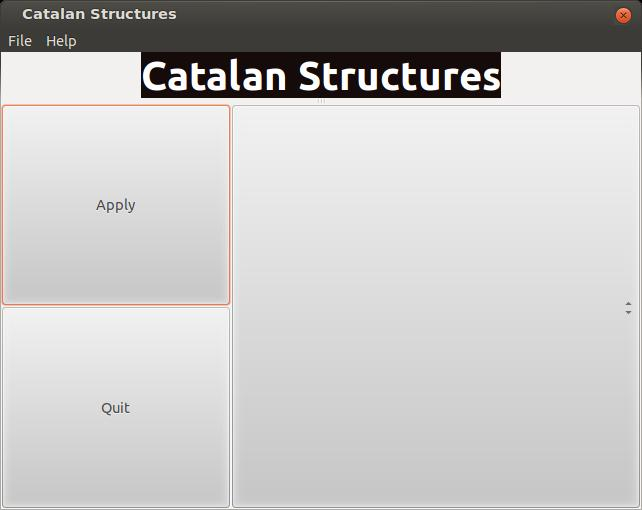
\includegraphics[width=90mm]{mainGUIScreenshot.jpeg}\\
\caption{Modelled using Glade \cite{Glade}}}\\
\\
To build this main interface, the user interface design software, Glade, was used for modelling and the Gtk bindings for Haskell were used to implement each action from the interface. To model the interface I adopted the standard method for modelling any user inface with Glade and Haskell, it is as follows:
\begin{lstlisting}
main :: IO ()
main = do
	initGUI 
	
	builder <- initBuilder

	<Omitted content>

	widgetShowAll main_window
	mainGUI 
\end{lstlisting}
In the above code, we define the function {\it main} which is of type {\it IO ()}. Within the main body of the function, using the IO monad we sequentially carry out a number of actions. Firstly we initalise the GUI toolkit for Haskell's Gtk bindings, and create a builder. To create the builder used for our user interface we define the function {\it initBuilder}.
\begin{lstlisting}
initBuilder :: IO Builder
initBuilder = do
	builder <- builderNew 
	builderAddFromFile builder "mainGui.glade" 
	return builder
\end{lstlisting}
In the {\it initBuilder} function, we create a new builder using the function {\it builderNew} and then add the user interfaces {\it .glade} file to the builder and finally return the builder.\\
Continuing with the function main, to end the function we explicitly tell the program to show the main window, denoted here as {\it main\_window} and then call mainGUI to run the main GUI loop and continue the program until it is terminated by the user. The omitted code will be discussed later in this section.


%%%%%%%%%%%%%%%%%%%%%%%%%%%%%%%%%%%%%%%%%%%%%%%%%%%%%%%%%%%%%%%%%%%%%%%%%%%%%%%%%%%
%	Combinatorial Statistics
%%%%%%%%%%%%%%%%%%%%%%%%%%%%%%%%%%%%%%%%%%%%%%%%%%%%%%%%%%%%%%%%%%%%%%%%%%%%%%%%%%%
\section{Bijections}
In this chapter we will discuss each bijection: how they function and how they biject functions.\\
\subsection{132-avoiding permutation to Dyck path}
Knuth\cite{KnuthVol1} gives a bijection from 312-avoiding permutations. By taking the complement of 312, it is a bijection form 132-avoiding permutations to Dyck paths.\\
We are by describing the bijection from 132-avoiding permutations to Dyck Paths. Henceforth this will be described as the bijection between Dyck paths and 132-avoiding permutations.\\ 
Let $\sigma$ = $\alpha n\beta$ be a 132-avoiding permutation of length $n$. As we saw in the proof of One Stack Sortable Permutations, every element of $\alpha$ is larger than every element of $\beta$ or else a 132 pattern would be formed by the permutation.\\
When converting between 132-avoiding permutations and Dyck paths we use the encodings that we formulated when defining Dyck paths. These are up $\rightarrow u$ and down $\rightarrow d$.
We define the bijection between Dyck paths and 132-avoiding permutations recursively by:\\
\begin{equation}
\begin{split}
& $f(\sigma) = u f(\alpha) d f(\beta)$ and $f(\epsilon) = \epsilon$\\
\end{split}
\end{equation}
where $\epsilon$ is the empty word, or permutation. Therefore by the bijection between Dyck paths and 132-avoiding permutations, the position of the largest element in a 132-avoiding permutation determines the first to return to the $x$-axis and vice versa.\\


\subsubsection{Examples of 132-avoiding permutation to Dyck path}
\subsubsubsection{Example 1}
Let $\sigma = 2134$.\\
Now we must calculate $f(\sigma)$.\\
\begin{equation}
\begin{split}
& $ f(\sigma) $ = $ f(2134) $\\
& = $ u f(213) d $\\
& = $ uu f(21) dd $\\
& = $ uuududdd $\\
\end{split}
\end{equation}
Hence the corresponding Dyck path for the permutation $2134$ has the encoding $uuududdd$.

\subsubsubsection{Example 2}
Let $\pi = 7564213$.\\
Now we must calculate $f(\pi)$.\\
\begin{equation}
\begin{split}
& $ f(\pi) $ = $ f(7654213) $\\
& = $ ud f(564213) $\\
& = $ udu f(5) d f(4213) $\\
& = $ uduuddud f(213) $\\
& = $ uduuddudu f(21) d $\\
& = $ uduudduduududd $ \\
\end{split}
\end{equation}
Hence the corresponding Dyck path for the permutation $7654213$ has the encoding $uduudduduududd$.

\subsection{Dyck path to 132-avoiding permutation}
To solve the problem of converting a Dyck Path to a 132-avoiding permutation we will use the Robinson-Schensted-Knuth correspondence.\\
Given a 132-avoiding permutation we will start by applying the Robinson-Schensted-Knuth correspondence (RSK-correspondence) to the permutation. As is known the RSK-correspondence gives a bijection between a permutation $\sigma$ of length $n$ and pairs ($P$, $Q$) of {\it standard Young tableaux} of the same shape $\lambda$  $\vdash$ $n$, hence for 132-avoiding permutations Young tableau has at most two rows.\\
The {\it insertion tableau}, $P$, is obtained by reading in the permutation $\sigma$ = $a_{1}a_{2}...a_{n}$ left to right and inserting the element of the permutation into the partial tableau that has already been obtained by using Schensted's insertion algorithm. Assume that $a_{1}a_{2}...a_{i-1}$ have already been inserted. If $a_{i}$ is larger than all the elements of the first row of the tableau, place $a_{i}$ at the end of the first row of the tableau. If it is not, then let $m$ be the leftmost element in the first row that is larger than $a_{i}$, then place $a_{i}$ in the cell that is currently occupied by $m$ and move $m$ to the end of the second row.\\
The {\it recording tableau}, $Q$, is obtained by placing $i$, where $i$ is from $1$ to $n$, in the position of the cell that in the construction of $P$ was inserted at step $i$ (that is, the stage where $a_{i}$ was inserted).\\
$<$insert example$>$\\
Finally, to turn the pair of tableaux, ($P$, $Q$), into a Dyck path, $D$, we do it in two stages. Firstly, the first half, $X$ we get by recording, for $i$ from $1$ to $n$. If $i$ is in the first row of $P$ we record an up-step, $u$, and a down-step, $d$, if $i$ is in the second row of $P$. Let $Y$ be the word obtained by replacing all the $u$'s in $A$ with a $d$, and all the $d$'s in $A$ with a $u$, then $D$ = $XY^r$ where $Y^r$ is the reverse of $Y$.\\
$<$insert example$>$


%%%%%%%%%%%%%%%%%%%%%%%%%%%%%%%%%%%%%%%%%%%%%%%%%%%%%%%%%%%%%%%%%%%%%%%%%%%%%%%%%%%
%	Combinatorial Statistics
%%%%%%%%%%%%%%%%%%%%%%%%%%%%%%%%%%%%%%%%%%%%%%%%%%%%%%%%%%%%%%%%%%%%%%%%%%%%%%%%%%%
\section{Combinatorial Statistics}
\subsection{Introduction}
A combinatorial statistic, $st$, is a mapping from a combinatorial structure, $\mathfrak{C}$, to an integer:\\
\centerline{$st: \mathfrak{C} \rightarrow \mathbb{Z}$}\\
In this chapter we will be discussing various combinatorial statistics which will lead to investigating which statistics are respected by each bijection evaluated in the next chapter.\\
The structures which we will be analysing bijections for are the structures which have been discussed in previous chapters.

\subsection{Permutation statistics}
In this section we will be focusing on the set of permutations on $\mathfrak{S}_n$. Our base set of statistics for permutations are:\\ \centerline{asc, des, exc, ldr, rdr, lir, rir, zeil, comp, lmax,}\\
\centerline{lmin, rmax, rmin, head, last, peak, valley, lds, lis, rank, cyc, fix}\\
The detailed explanation of each statistic in our base set is as follows:\\
asc: number of ascents: a letter $a_i$ such that $a_i < a_{i+1}$;\\
comp: number of components;\\
cyc: number of cycles;\\
des: number of descents: a letter $a_i$ such that $a_i > a_{i+1}$;\\
exc: number of excedences: positions $i$ such that $a_i > i$;\\
fix: number of fixed points: positions $i$ such that $a_i = i$;\\
head: first element of the permutation: $head(\pi) = a_1$;\\
last: last element of the permutation: $last(\pi) = a_n$;\\
ldr: length of the leftmost decreasing run;\\
lds: length of the leftmost decreasing subsequence;\\
lir: length of the leftmost increasing run;\\
lis: length of the leftmost increasing subsequence;\\
lmax: number of left to right maxima;\\
lmin: number of left to right minima;\\
peak: number of peaks: positions $i$ in $\pi$ such that $a_{i-1} < a_i > a_{i+1}$;\\
rmax: number of right to left maxima;\\
rank: largest $k$ such that $a_i > k$ for all $i \leq k$;\\
rdr: length of the rightmost decreasing run;\\
rir: length of the rightmost increasing run;\\
rmin: number of right to left minima\\
valley: number of valleys: positions $i$ in $\pi$ such that $a_{i-1} > a_i < a_{i+1}$;\\
zeil: length of the longest sub-word $n(n-1)...i$.\\

\subsection{Dyck Path statistics}
In this section we will be focusing on the set of Dyck Paths, $\mathfrak_{D}$. Our base set of statistics for Dyck Paths are:\\ \centerline{ups, downs, returns, peaks, heights}\\
The detailed explanation of each statistic is as follows:\\
downs: number of down-steps;\\
heights: the highest point of $\mathfrak_{D}$;\\
maj: major index: the sum of the positions of the valleys of $\mathfrak_{D}$.
noDoubleRises: number of double rises: how many consecutive up steps in $\mathfrak_{D}$.\\
noInitRises: number of initial rises: how many consecutive up steps in $\mathfrak_{D}$ from $(0,0)$.\\
peaks: number of peaks in $\mathfrak_{D}$;\\
returns: number of times the path returns to the x-axis: how many times $\mathfrak_{D}$ touches $x=0$;\\
ups: number of up-steps.\\

\subsection{Young Tableaux statistics}

\subsection{$n+2$-gon statistics}

\subsection{Mapping of statistics}
For each statistic, we will define a mapping, $f$, such that every statistic for each structure will correspond to a statistic for each other structure:\\
\centerline{$f: stat_1({\mathfrak_{C}}) \rightarrow stat_2(\phi(\mathfrak_{C}))$}\\
When discussing which mappings will be used to show equivalent statistic sets between structures we will use the format $stat_1 \simeq stat_2$ where $\phi$ is the bijection under consideration.

\subsubsection{Permutations $\rightarrow$ Dyck Paths}
The correspondence between permutation statistics and Dyck Path statistics will be defined as follows:


%%%%%%%%%%%%%%%%%%%%%%%%%%%%%%%%%%%%%%%%%%%%%%%%%%%%%%%%%%%%%%%%%%%%%%%%%%%%%%%%%%%%%%%%%%%%%%%%%%%%%%%%
%	Analysis of Bijections
%%%%%%%%%%%%%%%%%%%%%%%%%%%%%%%%%%%%%%%%%%%%%%%%%%%%%%%%%%%%%%%%%%%%%%%%%%%%%%%%%%%%%%%%%%%%%%%%%%%%%%%%
\section{Analysis of Bijections}
In this chapter we will be looking at the analysis for each bijection over a given test data then prove the equivalence of each statistic by using the equidistribution theorem. Each statistic value will have an error value of $\pm 1$.

\subsection{Equidistribution theorem}
For two sets of Catalan structures $\mathcal_{A}$ and $\mathcal_{B}$, with their respective statistic sets $s_1, s_2,..., s_k$ and $t_1, t_2,...,t_l$. Then $s$ and $t$ are said to be equidistributed if $F = G$ where $F = {\sum_{a \in {\mathcal_{A}}n}} x^{s(a)}$ and $G = {\sum_{b \in {\mathcal_{A}}_n}} x^{t(b)}$. The coefficient of each set is given by $[x^k]F = \#\{a \in {\mathcal_{A}} : S(a) = k\}$.

\subsection{Standard Bijection}
For the standard bijection we will look at an analysis of equidistribution over many permutations which are in table~\ref{table:StandardPerms}. 

\subsubsection{Analysis of equidistribution of Standard bijection over many permutations}
From the findings in ~\ref{table:StandardPerms1} we can see that all of our base set of statistics are respected. Categorising the statistics for each set of results, the equidistribution value was recorded in table~\ref{table:StandardPerms1} and the equidistribution of statistics is shown in table~\ref{table:EDStandardPerms} and table~\ref{table:EDStandardDP}. We find from table~\ref{table:EDStandardPerms} and table~\ref{table:EDStandardDP} that the statistics: comp, cyc, and peak are equidistributed over the value $0$; asc, des, fix, lir, lis, rank, rdr, noDoubleRises, and returns are equidistributed over the value $1$; exc, head, last, ldr, lds, lmax, lmin, rmax, rir, rmin, zeil, heights, and peaks are equidistributed over the value $2$; and finally, downs, noInitRises, and ups are equidistributed over the value $3$. To show which statistics correspond to each other fully we can look at the table below. For the purposes of table~\ref{table:FinalEDStandard}, \#ED will correspond to the equidistribution group, SSP Stats will correspond to the statistics for stack sortable permutations and Dyck Path Stats will correspond to the statistics for Dyck Paths.
\begin{table}[H]
\caption{Simion-Schmidt results over base set statistics.}
\begin{tabular}{c | c | c}
\hline\hline
\#ED & SSP Stats & Dyck Path Stats\\ [0.5ex]
\hline
0 & comp, cyc, peak & - \\
\hline
1 & asc, des, fix, lir, lis, rank, rdr & noDoubleRises, returns \\
\hline
2 & exc, head, last, ldr, lds, lmax, lmin, rmax, rir, rmin, zeil & heights, peaks \\
\hline
3 & - & downs, noInitRises, ups\\
\hline
\end{tabular}
\label{table:FinalEDStandard}
\end{table}
Currently no equidistribution can be made for the statistics valley, and maj as they have returned inconclusive results in table~\ref{table:StandardPerms1}.

\subsection{Simion Schmidt Bijection}
For the Simion-Schmidt bijection, we will start with the following permutation: $\pi_1 = 6743152$.\\
From the Simion-Schmidt bijection, $Simion-Schmidt(\pi_1) = 6743125$.\\
\subsubsection{Analysis of Simion-Schmidt bijection where $\pi = 6743152$}
From the findings in ~\ref{table:simionschmidt1} we can see that all of our base set of statistics are respected except from the last element of the permutation and the rightmost increasing run of the permutation.\\
Analysing the permutation further we shall investigate why this is the case. As the Simion-Schmidt bijection has changed the last two letters of $\pi_1$ to convert $\pi_1$ from a $123$-avoiding permutation to a $132$-avoiding permutation it follows in this case that the last two letters will change since $152$ avoids $123$ whereas $152$ does not avoid 132 and $125$ avoids $132$ but does not avoid $123$.\\
Now let's look at the rightmost increasing runs: for $\pi_1$ they are: $7431$, $431$, $74$, $31$ and $52$. For $Simion-Schmidt(\pi_1)$ they are:  $7431$, $431$, $74$, $31$, $125$, and $12$. Comparing these values the differing values for $\pi_1$ are $52$ and the differing values for $Simion-Schmidt(\pi_1)$ are $125$ and $12$. Hence from the bijection these two statistics should not be respected for this particular permutation. 
\subsubsection{Analysis of equidistribution of Simion Schmidt bijection over many permutations}
To find an approximate equidistribution for the Simion-Schmidt bijection, we will be looking at the permutations in table~\ref{table:SSPerms} on page~\pageref{table:SSPerms}. Categorising the statistics for the 3 sets of results, we find from our results in table~\ref{table:SSPerms1} on page~\pageref{table:SSPerms1}, and our final equidistribution in table~\ref{table:EDSSPerms} on page~\pageref{table:EDSSPerms} that the statistics: comp cyc, fix, and peak are equidistributed over the value $0$; asc, des, exc, lir, lis, lmax, rank, rdr, valley, and zeil are equidistributed over the value $1$; last, ldr, lds, lmin, rmax, rir, and rmin are equidistributed over the value $2$; and finally that the statistic head does not have a statistic which is is equidistributed with.

\subsubsection{Analysis of equidistribution of Fulmek bijection over many permutations}
To find an approximate equidistribution for the Simion-Schmidt bijection, we will be looking at the permutations in table~\ref{table:FulmekPerms} on page~\pageref{table:FulmekPerms}. Categorising the statistics for the four sets of results, we find from our results in table~\ref{table:FulmekPerms1} on page~\pageref{table:FulmekPerms1}, and our final equidistribution in table~\ref{table:EDFulmekPerms} that the statistics: comp and cyc are equidistributed over the value $0$; asc, last, ldr, lis, peak, rir, rmin, and valley are equidistributed over the value $1$; des, exc, lds, lmax, rank and rdr are equidistributed over the value $2$; head and zeil are equidistributed over the value $3$. It was found that the statistics lmin and rmax are equidistributed over the value $2$ or the value $3$ with the data we have. It was found also that the statistics fix and lir are not equidistributed with any other value. 
%%%%%%%%%%%%%%%%%%%%%%%%%%%%%%%%%%%%%%%%%%%%%%%%%%%%%%%%%%%%%%%%%%%%%%%%%%%%%%%%%%%%%%%%%%%%%%%%%%%%%%%%
%	References
%%%%%%%%%%%%%%%%%%%%%%%%%%%%%%%%%%%%%%%%%%%%%%%%%%%%%%%%%%%%%%%%%%%%%%%%%%%%%%%%%%%%%%%%%%%%%%%%%%%%%%%%

\newpage
\bibliographystyle{amsplain}
\bibliography{CatalanStructuresBib}

%%%%%%%%%%%%%%%%%%%%%%%%%%%%%%%%%%%%%%%%%%%%%%%%%%%%%%%%%%%%%%%%%%%%%%%%%%%%%%%%%%%%%%%%%%%%%%%%%%%%%%%%
%	Appendix 1 - tables of data
%%%%%%%%%%%%%%%%%%%%%%%%%%%%%%%%%%%%%%%%%%%%%%%%%%%%%%%%%%%%%%%%%%%%%%%%%%%%%%%%%%%%%%%%%%%%%%%%%%%%%%%%
\newpage
\section{Appendix 1: Tables of data}
\begin{table}[H]
\caption{Simion-Schmidt results over base set statistics.}
\centering
\begin{tabular}{c | c c c}
\hline\hline
Statistic & $\pi_1$ & $ss(\pi_1)$ & Difference \\ [0.5ex]
\hline
asc & 2 & 3 & -1 \\ 
comp & 0 & 0 & 0 \\
cyc & 0 & 0 & 0 \\
des & 4 & 3 & 1 \\
exc & 3 & 3 & 0 \\
fix & 0 & 0 & 0 \\
head & 6 & 6 & 0 \\
last & 2 & 5 & -3 \\
ldr & 1 & 1 & 0 \\
lds & 5 & 4 & 1 \\
lir & 2 & 2 & 0 \\
lis & 4 & 4 & 0 \\
lmax & 2 & 2 & 0 \\
lmin & 4 & 4 & 0 \\
peak & 2 & 1 & 0 \\
rmax & 3 & 2 & 1 \\
rank & 3 & 3 & 0 \\
rdr & 2 & 1 & 0 \\
rir & 1 & 3 & -2 \\
rmin & 2 & 3 & -1 \\
valley & 1 & 1 & 0 \\
zeil & 2 & 2 & 0 \\
\hline
\end{tabular}
\label{table:simionschmidt1}
\end{table}
\newpage

\begin{table}[H]
\caption{Permutations for Standard bijection analysis}
\centering
\begin{tabular}{c | c c}
\hline\hline
n & $\pi_n$ & $\phi(\pi_n)$ \\ [0.5ex]
\hline
1 & 123 & [U,U,U,D,D,D] \\
2 & 213 & [U,U,D,U,D,D] \\
3 & 321 & [U,D,U,D,U,D] \\
4 & 312 & [U,D,U,U,D,D] \\
5 & 2134 & [U,U,U,D,U,D,D,D] \\
6 & 4321 & [U,D,U,D,U,D,U,D] \\
\hline
\end{tabular}
\label{table:StandardPerms}
\end{table}
%\newpage

\begin{table}[H]
\caption{Permutations for Simion-Schmidt bijection analysis}
\centering
\begin{tabular}{c | c c}
\hline\hline
n & $\pi_n$ & $ss(\pi_n)$ \\ [0.5ex]
\hline
1 & 312 & 412 \\
2 & 132 & 123 \\
3 & 312 & 412 \\
\hline
\end{tabular}
\label{table:SSPerms}
\end{table}
%\newpage

\begin{table}[H]
\caption{Permutations for Fulmek bijection analysis}
\centering
\begin{tabular}{c | c c}
\hline\hline
n & $\pi_n$ & $fulmek(\pi_n)$ \\ [0.5ex]
\hline
1 & 312 & 321 \\
2 & 2413 & 2431\\
3 & 3412 & 3421\\
4 & 3142 & 3241\\
\hline
\end{tabular}
\label{table:FulmekPerms}
\end{table}
\newpage
%%%%%%%%%%%%%%%%%%%%%%%%%%%%%%%%%%%%
%Statistic tables for above tables
%%%%%%%%%%%%%%%%%%%%%%%%%%%%%%%%%%%%

%%%%%%%%%%%%%%%%%%%%%%%%%%%%%%%%%%%%%%%%%%%%%%%%%%%%%%%%%%%%

%([[(2,"asc"),(0,"comp"),(0,"cyc"),(0,"des"),(3,"exc"),(3,"fix"),(1,"head"),(3,"last"),(1,"ldr"),(0,"lds"),(3,"lir"),(2,"lis"),(3,"lmax"),(1,"lmin"),(0,"peak"),(1,"rmax"),(1,"rank"),(1,"rdr"),(3,"rir"),(3,"rmin"),(0,"valley"),(1,"zeil")]],
%
%[[(3,"uCnt"),(3,"dCnt"),(1,"returnsXAxis"),(1,"peaks"),(3,"heightStat"),(2,"noInitialRises"),(2,"noDoubleRises"),(3,"majorIndex")]])
%%%%%%%%%%%%%%%%%%%%%%%%%%%%%%%%%%%%%%%%%%%%%%%%%%%%%%%%%%%%
% $pi_2$ & standard(pi_2)
% ([[(1,"asc"),(0,"comp"),(0,"cyc"),(1,"des"),(2,"exc"),(1,"fix"),(2,"head"),(3,"last"),(2,"ldr"),(2,"lds"),(1,"lir"),(1,"lis"),(2,"lmax"),(2,"lmin"),(0,"peak"),(1,"rmax"),(1,"rank"),(1,"rdr"),(2,"rir"),(2,"rmin"),(1,"valley"),(3,"zeil")]],
%
% [[(3,"dCnt"),(2,"heightStat"),(6,"majorIndex"),(1,"noDoubleRises"),(1,"noInitialRises"),(2,"peaks"),(1,"returnsXAxis"),(3,"uCnt")]])
%%%%%%%%%%%%%%%%%%%%%%%%%%%%%%%%%%%%%%%%%%%%%%%%%%%%%%%%%%%%%%
% $pi_3$ & standard(pi_3)
%([[(0,"asc"),(0,"comp"),(0,"cyc"),(2,"des"),(2,"exc"),(1,"fix"),(3,"head"),(1,"last"),(3,"ldr"),(2,"lds"),(1,"lir"),(0,"lis"),(1,"lmax"),(3,"lmin"),(0,"peak"),(3,"rmax"),(2,"rank"),(3,"rdr"),(1,"rir"),(1,"rmin"),(0,"valley"),(3,"zeil")]],
%
%[[(3,"dCnt"),(1,"heightStat"),(9,"majorIndex"),(0,"noDoubleRises"),(3,"noInitialRises"),(3,"peaks"),(3,"returnsXAxis"),(3,"uCnt")]])
%%%%%%%%%%%%%%%%%%%%%%%%%%%%%%%%%%%%%%%%%%%%%%%%%%%%%%%%%%%%%%
% $pi_4$ & standard(pi_4)
%([[(1,"asc"),(0,"comp"),(0,"cyc"),(1,"des"),(1,"exc"),(0,"fix"),(3,"head"),(2,"last"),(2,"ldr"),(2,"lds"),(1,"lir"),(1,"lis"),(1,"lmax"),(2,"lmin"),(0,"peak"),(2,"rmax"),(1,"rank"),(1,"rdr"),(2,"rir"),(2,"rmin"),(1,"valley"),(1,"zeil")]],
%[[(3,"dCnt"),(2,"heightStat"),(5,"majorIndex"),(1,"noDoubleRises"),(2,"noInitialRises"),(2,"peaks"),(2,"returnsXAxis"),(3,"uCnt")]])
%%%%%%%%%%%%%%%%%%%%%%%%%%%%%%%%%%%%%%%%%%%%%%%%%%%%%%%%%%%%%%
% $pi_5$ & standard(pi_5)
%([[(2,"asc"),(0,"comp"),(0,"cyc"),(1,"des"),(3,"exc"),(2,"fix"),(2,"head"),(4,"last"),(2,"ldr"),(2,"lds"),(1,"lir"),(2,"lis"),(3,"lmax"),(2,"lmin"),(0,"peak"),(1,"rmax"),(1,"rank"),(1,"rdr"),(3,"rir"),(3,"rmin"),(1,"valley"),(1,"zeil")]],
%[[(4,"dCnt"),(3,"heightStat"),(8,"majorIndex"),(2,"noDoubleRises"),(3,"noInitialRises"),(2,"peaks"),(1,"returnsXAxis"),(4,"uCnt")]])
%%%%%%%%%%%%%%%%%%%%%%%%%%%%%%%%%%%%%%%%%%%%%%%%%%%%%%%%%%%%%%
% $pi_6$ & standard(pi_6)
%([[(0,"asc"),(0,"comp"),(0,"cyc"),(3,"des"),(2,"exc"),(0,"fix"),(4,"head"),(1,"last"),(4,"ldr"),(3,"lds"),(1,"lir"),(0,"lis"),(1,"lmax"),(4,"lmin"),(0,"peak"),(4,"rmax"),(2,"rank"),(4,"rdr"),(1,"rir"),(1,"rmin"),(0,"valley"),(4,"zeil")]],
%[[(4,"dCnt"),(1,"heightStat"),(16,"majorIndex"),(0,"noDoubleRises"),(4,"noInitialRises"),(4,"peaks"),(4,"returnsXAxis"),(4,"uCnt")]])
%%%%%%%%%%%%%%%%%%%%%%%%%%%%%%%%%%%%%%%%%%%%%%%%%%%%%%%%%%%%%%
\begin{table}[H]
\caption{Statistics based upon table ~\ref{table:StandardPerms}}
\centering
\tabcolsep=0.11cm
\begin{tabular}{c | c c c c c c c c c c c c | c}
\hline\hline
Statistic & $\pi_1$ & $\phi(\pi_1)$ & $\pi_2$ & $\phi(\pi_2)$ & $\pi_3$ & $\phi(\pi_3)$ & $\pi_4$ & $\phi(\pi_4)$ & $\pi_5$ & $\phi(\pi_5)$ & $\pi_6$ & $\phi(\pi_6)$ & Eds value\\ [0.5ex]
\hline
asc & 2 & - & 1 & - & 0 & - & 1 & - & 2 & - & 0 & - & 1\\ 
comp & 0 & - & 0 & - & 0 & - & 0 & - & 0 & - & 0 & - & 0\\
cyc & 0 & - & 0 & - & 0 & - & 0 & - & 0 & - & 0 & - & 0\\
des & 0 & - & 1 & - & 2 & - & 1 & - & 1 & - & 3 & - & 1\\
exc & 3 & - & 2 & - & 2 & - & 1 & - & 3 & - & 2 & - & 2\\
fix & 3 & - & 1 & - & 1 & - & 0 & - & 2 & - & 0 & - & 1\\
head & 1 & - & 2 & - & 3 & - & 3 & - & 2 & - & 4 & - & 2\\
last & 3 & - & 3 & - & 1 & - & 2 & - & 4 & - & 1 & - & 2\\
ldr & 1 & - & 2 & - & 3 & - & 2 & - & 2 & - & 4 & - & 2\\
lds & 0 & - & 2 & - & 2 & - & 2 & - & 2 & - & 3 & - & 2\\
lir & 3 & - & 1 & - & 1 & - & 1 & - & 1 & - & 1 & - & 1\\
lis & 2 & - & 1 & - & 0 & - & 1 & - & 2 & - & 0 & - & 1\\
lmax & 3 & - & 2 & - & 1 & - & 1 & - & 3 & - & 1 & - & 2\\
lmin & 1 & - & 2 & - & 3 & - & 2 & - & 2 & - & 4 & - & 2\\
peak & 0 & - & 0 & - & 0 & - & 0 & - & 0 & - & 0 & - & 0\\
rmax & 1 & - & 1 & - & 3 & - & 2 & - & 1 & - & 4 & - & 2\\
rank & 1 & - & 1 & - & 2 & - & 1 & - & 1 & - & 2 & - & 1\\
rdr & 1 & - & 1 & - & 3 & - & 1 & - & 1 & - & 4 & - & 1\\
rir & 3 & - & 2 & - & 1 & - & 2 & - & 3 & - & 1 & - & 2\\
rmin & 3 & - & 2 & - & 1 & - & 2 & - & 3 & - & 1 & - & 2\\
valley & 0 & - & 1 & - & 0 & - & 1 & - & 1 & - & 0 & - & 0 or 1 (inconclusive)\\
zeil & 1 & - & 3 & - & 3 & - & 1 & - & 1 & - & 4 & - & 2\\
\hline
downs & - & 3 & - & 3 & - & 3 & - & 3 & - & 4 & - & 4 & 3\\
heights & - & 3 & - & 2 & - & 1 & - & 2 & - & 3 & - & 1 & 2\\
maj & - & 3 & - & 6 & - & 9 & - & 5 & - & 8 & - & 16 & inconclusive\\
noDoubleRises & - & 2 & - & 1 & - & 0 & - & 1 & - & 2 & - & 0 & 1\\
noInitRises & - & 2 & - & 1 & - & 3 & - & 2 & - & 3 & - & 4 & 3\\
peaks & - & 1 & - & 2 & - & 3 & - & 2 & - & 2 & - & 4 & 2\\
returns & - & 1 & - & 1 & - & 3 & - & 2 & - & 1 & - & 4 & 1\\
ups & - & 3 & - & 3 & - & 3 & - & 3 & - & 4 & - & 4 & 3\\
\hline
\end{tabular}
\label{table:StandardPerms1}
\end{table}
%%%%%%%%%%%%%%%%%%%%%%%%%%%%%%%%%%%%%%%%%%%%%%%%%%%%%%%%%%%%
% $\pi_1$
%[[(1,"asc"),(0,"comp"),(0,"cyc"),(1,"des"),(1,"exc"),(0,"fix"),(3,"head"),(2,"last"),(2,"ldr"),(2,"lds"),(1,"lir"),(1,"lis"),(1,"lmax"),(2,"lmin"),(0,"peak"),(2,"rmax"),(1,"rank"),(1,"rdr"),(2,"rir"),(2,"rmin"),(1,"valley"),(1,"zeil")],
%%%%%%%%%%%%%%%%%%%%%%%%%%%%%%%%%%%%%%%%%%
% $ss(\pi_1)
%[(1,"asc"),(0,"comp"),(0,"cyc"),(1,"des"),(1,"exc"),(0,"fix"),(4,"head"),(2,"last"),(2,"ldr"),(2,"lds"),(1,"lir"),(1,"lis"),(1,"lmax"),(2,"lmin"),(0,"peak"),(2,"rmax"),(1,"rank"),(1,"rdr"),(2,"rir"),(2,"rmin"),(1,"valley"),(1,"zeil")],[]]
%%%%%%%%%%%%%%%%%%%%%%%%%%%%%%%%%%%%%%%%%%%%%%%%%%%%%%%%%%%
% $\pi_2$
%[[(1,"asc"),(0,"comp"),(0,"cyc"),(1,"des"),(2,"exc"),(1,"fix"),(1,"head"),(2,"last"),(1,"ldr"),(1,"lds"),(2,"lir"),(2,"lis"),(2,"lmax"),(1,"lmin"),(1,"peak"),(2,"rmax"),(1,"rank"),(2,"rdr"),(1,"rir"),(2,"rmin"),(0,"valley"),(1,"zeil")],
%%%%%%%%%%%%%%%%%%%%%%%%%%%%%%%%%%%%%%%%%%
% $ss(\pi_2)$
%[(2,"asc"),(0,"comp"),(0,"cyc"),(0,"des"),(3,"exc"),(3,"fix"),(1,"head"),(3,"last"),(1,"ldr"),(0,"lds"),(3,"lir"),(2,"lis"),(3,"lmax"),(1,"lmin"),(0,"peak"),(1,"rmax"),(1,"rank"),(1,"rdr"),(3,"rir"),(3,"rmin"),(0,"valley"),(1,"zeil")],[]]
%%%%%%%%%%%%%%%%%%%%%%%%%%%%%%%%%%%%%%%%%%%%%%%%%%%%%%%%%%%
% $\pi_3$
%[[(1,"asc"),(0,"comp"),(0,"cyc"),(1,"des"),(1,"exc"),(0,"fix"),(3,"head"),(2,"last"),(2,"ldr"),(2,"lds"),(1,"lir"),(1,"lis"),(1,"lmax"),(2,"lmin"),(0,"peak"),(2,"rmax"),(1,"rank"),(1,"rdr"),(2,"rir"),(2,"rmin"),(1,"valley"),(1,"zeil")],
%%%%%%%%%%%%%%%%%%%%%%%%%%%%%%%%%%%%%%%%%%
% $ss(\pi_3)$
%[(1,"asc"),(0,"comp"),(0,"cyc"),(1,"des"),(1,"exc"),(0,"fix"),(4,"head"),(2,"last"),(2,"ldr"),(2,"lds"),(1,"lir"),(1,"lis"),(1,"lmax"),(2,"lmin"),(0,"peak"),(2,"rmax"),(1,"rank"),(1,"rdr"),(2,"rir"),(2,"rmin"),(1,"valley"),(1,"zeil")],[]]
%%%%%%%%%%%%%%%%%%%%%%%%%%%%%%%%%%%%%%%%%%%%%%%%%%%%%%%%%%%
\begin{table}[H]
\caption{Statistics based upon table ~\ref{table:SSPerms}}
\centering
\begin{tabular}{c | c c c c c c c | c}
\hline\hline
Statistic & $\pi_1$ & $ss(\pi_1)$ & $\pi_2$ & $ss(\pi_2)$ & $\pi_3$ & $ss(\pi_3)$ & Mean & Equidistribution value\\ [0.5ex]
\hline
asc & 1 & 1 & 1 & 2 & 1 & 1 & 1.167 & 1\\ 
comp & 0 & 0 & 0 & 0 & 0 & 0 & 0 & 0\\
cyc & 0 & 0 & 0 & 0 & 0 & 0 & 0 & 0\\
des & 1 & 1 & 1 & 0 & 1 & 1 & 0.83 & 1\\
exc & 1 & 1 & 2 & 3 & 1 & 1 & 1.5 & 1\\
fix & 0 & 0 & 1 & 3 & 0 & 0 & 0.67 & 0\\
head & 3 & 4 & 1 & 1 & 3 & 4 & 2.67 & 3\\
last & 2 & 2 & 2 & 3 & 2 & 2 & 2.167 & 2\\
ldr & 2 & 2 & 1 & 1 & 2 & 2 & 1.67 & 2\\
lds & 2 & 2 & 1 & 0 & 2 & 2 & 1.5 & 2\\
lir & 1 & 1 & 2 & 3 & 1 & 1 & 1.5 & 1\\
lis & 1 & 1 & 2 & 2 & 1 & 1 & 1.33 & 1\\
lmax & 1 & 1 & 2 & 3 & 1 & 1 & 1.5 & 1\\
lmin & 2 & 2 & 1 & 1 & 2 & 2 & 1.67 & 2\\
peak & 0 & 0 & 1 & 0 & 0 & 0 & 0.5 & 0\\
rmax & 2 & 2 & 2 & 1 & 2 & 2 & 1.83 & 2\\
rank & 1 & 1 & 1 & 1 & 1 & 1 & 1 & 1\\
rdr & 1 & 1 & 2 & 1 & 1 & 1 & 1.167 & 1\\
rir & 2 & 2 & 1 & 3 & 2 & 2 & 1.67 & 2\\
rmin & 2 & 2 & 2 & 3 & 2 & 2 & 2.167 & 2\\
valley & 1 & 1 & 0 & 0 & 1 & 1 & 0.5 & 1\\
zeil & 1 & 1 & 1 & 1 & 1 & 1 & 1 & 1\\
\hline
\end{tabular}
\label{table:SSPerms1}
\end{table}
%\newpage
%%%%%%%%%%%%%%%%%%%%%%%%%%%%%%%%%%%%%%%%%%%%%%%%%%%%%%%%%%%%
% $\pi_1$
%([[(0,"asc"),(0,"comp"),(0,"cyc"),(2,"des"),(2,"exc"),(1,"fix"),(3,"head"),(1,"last"),(3,"ldr"),(2,"lds"),(1,"lir"),(0,"lis"),(1,"lmax"),(3,"lmin"),(0,"peak"),(3,"rmax"),(2,"rank"),(3,"rdr"),(1,"rir"),(1,"rmin"),(0,"valley"),(3,"zeil")]],
%%%%%%%%%%%%%%%%%%%%%%%%%%%%%%%%%%%%%%%%%%
% $fk(\pi_1)
%(0,"asc"),(0,"comp"),(0,"cyc"),(2,"des"),(2,"exc"),(1,"fix"),(3,"head"),(1,"last"),(3,"ldr"),(2,"lds"),(1,"lir"),(0,"lis"),(1,"lmax"),(3,"lmin"),(0,"peak"),(3,"rmax"),(2,"rank"),(3,"rdr"),(1,"rir"),(1,"rmin"),(0,"valley"),(3,"zeil")]])
%%%%%%%%%%%%%%%%%%%%%%%%%%%%%%%%%%%%%%%%%%%%%%%%%%%%%%%%%%%
% $\pi_2$
%([[(2,"asc"),(0,"comp"),(0,"cyc"),(1,"des"),(2,"exc"),(0,"fix"),(2,"head"),(3,"last"),(1,"ldr"),(2,"lds"),(2,"lir"),(3,"lis"),(2,"lmax"),(2,"lmin"),(1,"peak"),(2,"rmax"),(2,"rank"),(1,"rdr"),(2,"rir"),(2,"rmin"),(1,"valley"),(1,"zeil")]],
%%%%%%%%%%%%%%%%%%%%%%%%%%%%%%%%%%%%%%%%%%
% $fk(\pi_2)$
%(1,"asc"),(0,"comp"),(0,"cyc"),(2,"des"),(3,"exc"),(1,"fix"),(2,"head"),(1,"last"),(1,"ldr"),(2,"lds"),(2,"lir"),(2,"lis"),(2,"lmax"),(2,"lmin"),(1,"peak"),(3,"rmax"),(2,"rank"),(3,"rdr"),(1,"rir"),(1,"rmin"),(0,"valley"),(1,"zeil")]])
%%%%%%%%%%%%%%%%%%%%%%%%%%%%%%%%%%%%%%%%%%%%%%%%%%%%%%%%%%%
% $\pi_3$
%([[(2,"asc"),(0,"comp"),(0,"cyc"),(1,"des"),(2,"exc"),(0,"fix"),(3,"head"),(2,"last"),(1,"ldr"),(2,"lds"),(2,"lir"),(3,"lis"),(2,"lmax"),(2,"lmin"),(1,"peak"),(2,"rmax"),(2,"rank"),(1,"rdr"),(2,"rir"),(2,"rmin"),(1,"valley"),(2,"zeil")]],
%%%%%%%%%%%%%%%%%%%%%%%%%%%%%%%%%%%%%%%%%%
% $fk(\pi_3)$
%[[(1,"asc"),(0,"comp"),(0,"cyc"),(2,"des"),(2,"exc"),(0,"fix"),(3,"head"),(1,"last"),(1,"ldr"),(2,"lds"),(2,"lir"),(2,"lis"),(2,"lmax"),(3,"lmin"),(1,"peak"),(3,"rmax"),(2,"rank"),(3,"rdr"),(1,"rir"),(1,"rmin"),(0,"valley"),(4,"zeil")]])
%%%%%%%%%%%%%%%%%%%%%%%%%%%%%%%%%%%%%%%%%%%%%%%%%%%%%%%%%%%
% $\pi_4$
%([[(1,"asc"),(0,"comp"),(0,"cyc"),(2,"des"),(2,"exc"),(0,"fix"),(3,"head"),(2,"last"),(2,"ldr"),(3,"lds"),(1,"lir"),(2,"lis"),(2,"lmax"),(2,"lmin"),(1,"peak"),(2,"rmax"),(1,"rank"),(2,"rdr"),(1,"rir"),(2,"rmin"),(1,"valley"),(2,"zeil")]],
%%%%%%%%%%%%%%%%%%%%%%%%%%%%%%%%%%%%%%%%%%
% $fk(\pi_4)$
%[[(1,"asc"),(0,"comp"),(0,"cyc"),(2,"des"),(3,"exc"),(1,"fix"),(3,"head"),(1,"last"),(2,"ldr"),(3,"lds"),(1,"lir"),(2,"lis"),(2,"lmax"),(3,"lmin"),(1,"peak"),(2,"rmax"),(2,"rank"),(2,"rdr"),(1,"rir"),(1,"rmin"),(1,"valley"),(4,"zeil")]])
%%%%%%%%%%%%%%%%%%%%%%%%%%%%%%%%%%%%%%%%%%%%%%%%%%%%%%%%%%%
\begin{table}[H]
\caption{Statistics based upon table ~\ref{table:FulmekPerms}}
\centering
\begin{tabular}{c | c c c c c c c c | c}
\hline\hline
Statistic & $\pi_1$ & $fk(\pi_1)$ & $\pi_2$ & $fk(\pi_2)$ & $\pi_3$ & $fk(\pi_3)$ & $\pi_4$ & $fk(\pi_4)$ & Equidistribution\\ [0.5ex]
\hline
asc & 0 & 0 & 2 & 1 & 2 & 1 & 1 & 1 & 1\\ 
comp & 0 & 0 & 0 & 0 & 0 & 0 & 0 & 0 & 0\\
cyc & 0 & 0 & 0 & 0 & 0 & 0 & 0 & 0 & 0\\
des & 2 & 2 & 1 & 2 & 1 & 2 & 2 & 2 & 2\\
exc & 2 & 2 & 2 & 3 & 2 & 2 & 2 & 3 & 2\\
fix & 1 & 1 & 0 & 1 & 0 & 0 & 0 & 1 & 0 or 1 (inconclusive)\\
head & 3 & 3 & 2 & 2 & 3 & 3 & 3 & 3 & 3\\
last & 1 & 1 & 3 & 1 & 2 & 1 & 2 & 1 & 1\\
ldr & 3 & 3 & 1 & 1 & 1 & 1 & 2 & 2 & 1\\
lds & 2 & 2 & 2 & 2 & 2 & 2 & 3 & 3 & 2\\
lir & 1 & 1 & 2 & 2 & 2 & 2 & 1 & 1 & 1 or 2 (inconclusive)\\
lis & 0 & 0 & 3 & 2 & 3 & 2 & 2 & 2 & 1\\
lmax & 1 & 1 & 2 & 1 & 2 & 2 & 2 & 2 & 2\\
lmin & 3 & 3 & 2 & 2 & 2 & 3 & 2 & 3 & 2 or 3 (inconclusive)\\
peak & 0 & 0 & 1 & 1 & 1 & 1 & 1 & 1 & 1\\
rmax & 3 & 3 & 2 & 3 & 2 & 3 & 2 & 2 & 2 or 3 (inconclusive)\\
rank & 2 & 2 & 2 & 2 & 2 & 2 & 1 & 2 & 2\\
rdr & 3 & 3 & 1 & 3 & 1 & 3 & 2 & 2 & 2\\
rir & 1 & 1 & 2 & 1 & 2 & 1 & 1 & 1 & 1\\
rmin & 1 & 1 & 2 & 1 & 2 & 1 & 2 & 1 & 1\\
valley & 0 & 0 & 1 & 0 & 1 & 0 & 1 & 1 & 1\\
zeil & 3 & 3 & 1 & 1 & 2 & 4 & 2 & 4 & 3\\
\hline
\end{tabular}
\label{table:FulmekPerms1}
\end{table}
\newpage

%%%%%%%%%%%%%%%%%%%%%%%%%%%%%%%%%%%%%%%%%%%%%%%%%%%%%%%%%%%%
%Equidistrbution table Standard
%%%%%%%%%%%%%%%%%%%%%%%%%%%%%%%%%%%%%%%%%%%%%%%%%%%%%%%%%%%
\begin{table}[H]
\caption{Equidistribution for Standard bijection (permutations)}
\centering
\begin{tabular}{c | c}
\hline\hline
Statistic Group & List of Statistics \\ [0.5ex]
\hline
0 & {comp, cyc, peak, } \\
1 & {asc, des, fix, lir, lis, rank, rdr} \\
2 & {exc, head, last, ldr, lds, lmax, lmin, rmax, rir, rmin, zeil} \\
3 & {-} \\
\hline
\end{tabular}
\label{table:EDStandardPerms}
\end{table}

\begin{table}[H]
\caption{Equidistribution for Standard bijection (Dyck Paths)}
\centering
\begin{tabular}{c | c}
\hline\hline
Statistic Group & List of Statistics \\ [0.5ex]
\hline
0 & {-} \\
1 & {noDoubleRises, returns} \\
2 & {heights, peaks} \\
3 & {downs, noInitRises, ups} \\
\hline
\end{tabular}
\label{table:EDStandardDP}
\end{table}
\newpage

%%%%%%%%%%%%%%%%%%%%%%%%%%%%%%%%%%%%%%%%%%%%%%%%%%%%%%%%%%%%
%Equidistrbution table Simion-Schmidt
%%%%%%%%%%%%%%%%%%%%%%%%%%%%%%%%%%%%%%%%%%%%%%%%%%%%%%%%%%%
\begin{table}[H]
\caption{Equidistribution for Siimion-Schmidt bijection.}
\centering
\begin{tabular}{c | c}
\hline\hline
Statistic Group & List of Statistics \\ [0.5ex]
\hline
0 & {comp cyc, fix, peak} \\
1 & {asc, des, exc, lir, lis, lmax, rank, rdr, valley, zeil} \\
2 & {last, ldr, lds, lmin, rmax, rir, rmin} \\
3 & {head} 
\hline
\end{tabular}
\label{table:EDSSPerms}
\end{table}
\newpage

%%%%%%%%%%%%%%%%%%%%%%%%%%%%%%%%%%%%%%%%%%%%%%%%%%%%%%%%%%%%
%Equidistrbution table Fulmek
%%%%%%%%%%%%%%%%%%%%%%%%%%%%%%%%%%%%%%%%%%%%%%%%%%%%%%%%%%%
\begin{table}[H]
\caption{Equidistribution for Fulmek bijection.}
\centering
\begin{tabular}{c | c}
\hline\hline
Statistic Group & List of Statistics \\ [0.5ex]
\hline
0 & {comp cyc} \\
1 & {asc, last, ldr, lis, peak, rir, rmin, valley} \\
2 & {des, exc, lds, lmax, rank, rdr} \\
3 & {head, zeil} 
\hline
\end{tabular}
\label{table:EDFulmekPerms}
\end{table}
\newpage

\end{document}
